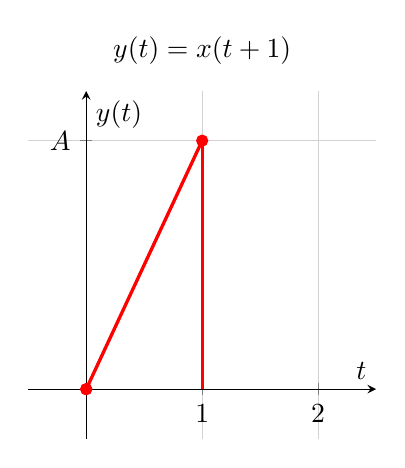
\begin{tikzpicture}
\begin{axis}[
    width=6cm,
    height=6cm,
    axis lines=middle,
    xlabel={$t$},
    ylabel={$y(t)$},
    title={$y(t) = x(t+1)$},
    xmin=-0.5, xmax=2.5,
    ymin=-0.2, ymax=1.2,
    xtick={0, 1, 2},
    ytick={1},
    yticklabels={$A$},
    grid=both,
    grid style={gray!15},
    major grid style={gray!35},
]

% Plot the advanced signal
\addplot[red, very thick, domain=0:1] {x};
\addplot[red, very thick] coordinates {(1,0) (1,1)};

% Add markers
\addplot[only marks, mark=*, mark size=2pt, red] coordinates {(0,0) (1,1)};
\addplot[only marks, mark=o, mark size=2pt, red] coordinates {(0,0)};

\end{axis}
\end{tikzpicture}

